% ==============================================================
%  Documentação do Cluster Heisenberg — CNPEM / Ilum
%  Compilar com: pdflatex heisenberg_doc.tex
% ==============================================================
\documentclass[11pt, a4paper]{article}

% --- Pacotes ---
% inputenc e fontenc substituídos por fontspec (XeTeX)
\usepackage[brazil]{babel}
\usepackage{lmodern}
\usepackage{geometry}
\usepackage{graphicx}
\usepackage{hyperref}
\usepackage{xcolor}
\usepackage{listings}
\usepackage{booktabs}
\usepackage{array}
\usepackage{longtable}
\usepackage{fancyhdr}
\usepackage{tcolorbox}
\usepackage{enumitem}
\usepackage{titlesec}
\usepackage{microtype}
\usepackage{float}
\usepackage{caption}
\usepackage{subcaption}
\usepackage{mdframed}
% fontawesome5 removido: causa crash no tectonic com fontes OTF
\usepackage{fontspec}
\usepackage{amssymb}

\geometry{
  top=2cm, bottom=2cm,
  left=2cm, right=2cm
}

% --- Cores ---
\definecolor{codeblue}{HTML}{1565C0}
\definecolor{codegray}{HTML}{F5F5F5}
\definecolor{codeborder}{HTML}{BDBDBD}
\definecolor{warnyellow}{HTML}{FFF8E1}
\definecolor{warnborder}{HTML}{F9A825}
\definecolor{tipgreen}{HTML}{E8F5E9}
\definecolor{tipborder}{HTML}{2E7D32}
\definecolor{infoblue}{HTML}{E3F2FD}
\definecolor{infoborder}{HTML}{1565C0}
\definecolor{dangerred}{HTML}{FFEBEE}
\definecolor{dangerborder}{HTML}{B71C1C}
\definecolor{heisenbergblue}{HTML}{0D3B6E}
\definecolor{accentblue}{HTML}{1976D2}

% --- Hyperlinks ---
\hypersetup{
  colorlinks=true,
  linkcolor=accentblue,
  urlcolor=accentblue,
  citecolor=accentblue,
  pdfauthor={CNPEM / Ilum},
  pdftitle={Documentação do Cluster Heisenberg},
}

% --- Estilo de código (terminal) ---
\lstdefinestyle{terminal}{
  backgroundcolor=\color{black},
  basicstyle=\ttfamily\small\color{white},
  breaklines=true,
  breakatwhitespace=false,
  keepspaces=true,
  showspaces=false,
  showstringspaces=false,
  frame=single,
  framerule=0.5pt,
  rulecolor=\color{codeborder},
  xleftmargin=8pt,
  xrightmargin=8pt,
  aboveskip=6pt,
  belowskip=6pt,
}

\lstdefinestyle{script}{
  backgroundcolor=\color{codegray},
  basicstyle=\ttfamily\small\color{black},
  keywordstyle=\color{codeblue}\bfseries,
  commentstyle=\color{gray}\itshape,
  breaklines=true,
  keepspaces=true,
  showspaces=false,
  showstringspaces=false,
  frame=single,
  framerule=0.5pt,
  rulecolor=\color{codeborder},
  xleftmargin=8pt,
  xrightmargin=8pt,
  aboveskip=6pt,
  belowskip=6pt,
  numbers=left,
  numberstyle=\tiny\color{gray},
  numbersep=8pt,
}

% --- Caixas de aviso ---
\tcbuselibrary{skins, breakable}

\newtcolorbox{dica}{
  colback=tipgreen, colframe=tipborder,
  title={$\star$\quad Dica},
  fonttitle=\bfseries, breakable
}
\newtcolorbox{atencao}{
  colback=warnyellow, colframe=warnborder,
  title={$\triangle$\quad Atenção},
  fonttitle=\bfseries, breakable
}
\newtcolorbox{info}{
  colback=infoblue, colframe=infoborder,
  title={$\circ$\quad Informação},
  fonttitle=\bfseries, breakable
}
\newtcolorbox{perigo}{
  colback=dangerred, colframe=dangerborder,
  title={$\times$\quad Cuidado},
  fonttitle=\bfseries, breakable
}

% --- Cabeçalho/rodapé ---
\pagestyle{fancy}
\fancyhf{}
\fancyhead[L]{\small\textcolor{heisenbergblue}{\textbf{Cluster Heisenberg}} --- CNPEM / Ilum}
\fancyhead[R]{\small\thepage}
\fancyfoot[C]{\small\textcolor{gray}{heisenberg.cnpem.br}}
\renewcommand{\headrulewidth}{0.4pt}
\renewcommand{\footrulewidth}{0.4pt}

% --- Títulos coloridos ---
\titleformat{\section}[block]
  {\Large\bfseries\color{heisenbergblue}}{{\thesection}}{0.8em}{}[\vspace{-0.3em}\rule{\linewidth}{0.8pt}]
\titleformat{\subsection}[block]
  {\large\bfseries\color{accentblue}}{\thesubsection}{0.7em}{}
\titleformat{\subsubsection}[block]
  {\normalsize\bfseries\color{accentblue}}{\thesubsubsection}{0.6em}{}

% --- Macros utilitárias ---
\newcommand{\cmd}[1]{\texttt{\textcolor{codeblue}{#1}}}
\newcommand{\placeholder}[1]{\textit{\textcolor{gray}{$\langle$#1$\rangle$}}}

% =====================================================================
\begin{document}
% =====================================================================

% --- Capa ---
\begin{titlepage}
  \centering
  \vspace*{1.5cm}

  
\includegraphics[width=0.35\textwidth]{images/ilum-logo.png}\\[1.5cm]

  {\Huge\bfseries\color{heisenbergblue} Cluster Heisenberg}\\[0.5cm]
  {\Large\color{accentblue} Guia do Usuário}\\[0.3cm]
  {\large\color{gray} Do Terminal ao Primeiro Job}\\[2cm]

  \begin{tcolorbox}[colback=infoblue, colframe=infoborder, width=0.75\textwidth]
    \centering
    \textbf{Endereço:} \texttt{heisenberg.cnpem.br}\\
    \textbf{Chamados:} \url{https://web-ilum.cnpem.br/chamado}\\
    \textbf{Reset de senha:} \texttt{http://172.20.10.15}
  \end{tcolorbox}

  \vfill
  {\large CNPEM --- Centro Nacional de Pesquisa em Energia e Materiais}\\
  {\large Ilum Escola de Ciência}\\[0.3cm]
  {\large\color{gray} Versão 1.0 --- Junho de 2026}
\end{titlepage}

% --- Sumário ---
\tableofcontents
\newpage

% =====================================================================
\section{Introdução ao Cluster Heisenberg}
% =====================================================================

O \textbf{Cluster Heisenberg} é a infraestrutura de computação de alto desempenho
(\textit{High-Performance Computing} --- HPC) disponibilizada pelo CNPEM para
pesquisadores e estudantes da Ilum. Com ele, você pode executar simulações,
análises de dados e treinamentos de modelos que seriam inviáveis em um computador
pessoal, pois o cluster distribui o trabalho entre dezenas de processadores e
placas de vídeo (GPUs) de forma coordenada.

\begin{info}
  O cluster utiliza o gerenciador de filas \textbf{Slurm} (\textit{Simple Linux
  Utility for Resource Management}) e o sistema de módulos \textbf{Environment
  Modules} para carregar softwares científicos. Ambos serão explicados em detalhe
  neste guia.
\end{info}

\subsection{Arquitetura Geral}

\begin{figure}[H]
  \centering
  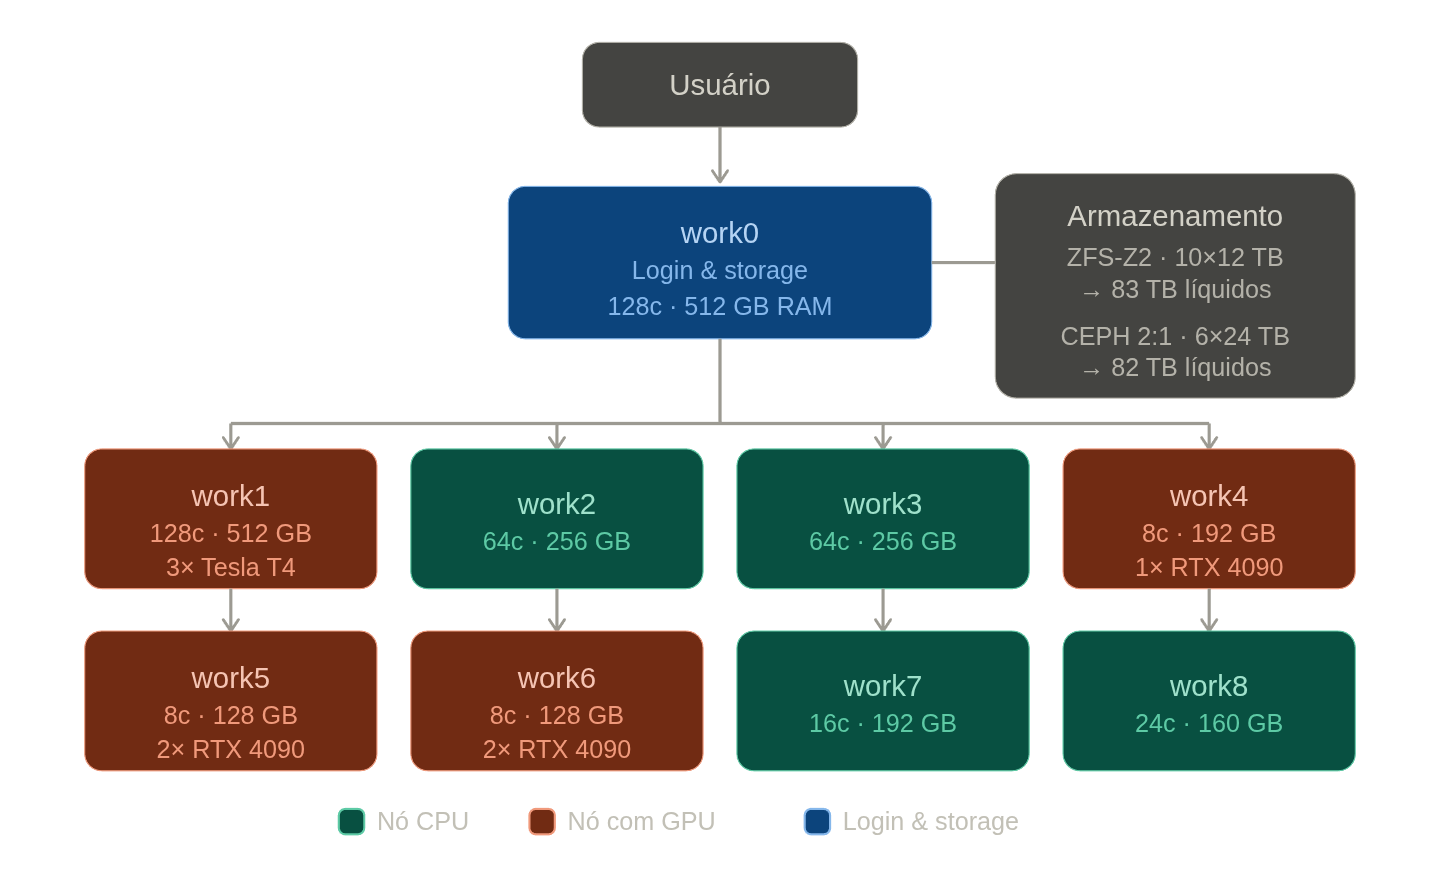
\includegraphics[width=0.85\textwidth]{images/Diagrama-Heisenberg.png}
  \caption{Arquitetura simplificada do Cluster Heisenberg.}
\end{figure}

O cluster é composto por:
\begin{itemize}
  \item \textbf{Nó de login (headnode):} \texttt{heisenberg.cnpem.br} ---
        o único ponto de acesso externo. É aqui que você faz login, edita
        scripts e submete jobs. \textbf{Não execute simulações pesadas
        diretamente nele.}
  \item \textbf{Nós de trabalho (\textit{worker nodes}):} \texttt{work0}
        a \texttt{work8} --- onde os jobs de fato rodam, gerenciados
        automaticamente pelo Slurm.
\end{itemize}

% =====================================================================
\section{Infraestrutura de Hardware}
% =====================================================================

\subsection{Nós de Trabalho}

A tabela abaixo resume o hardware de cada nó disponível no cluster.

\begin{longtable}{lrrrll}
  \toprule
  \textbf{Nó} & \textbf{CPUs} & \textbf{RAM (GB)} & \textbf{Sockets} & \textbf{GPU} & \textbf{Filas} \\
  \midrule
  \endhead
  work0 & 128 & 512 & 2 × 64 cores & --- & cpu \\
  work1 & 128 & 512 & 2 × 64 cores & 3 × NVIDIA T4 & cpu, gpu \\
  work2 &  64 & 256 & 2 × 32 cores & --- & cpu \\
  work3 &  64 & 256 & 2 × 32 cores & --- & cpu \\
  work4 &  8 & 128 & 1 × 16 cores & 1 × NVIDIA RTX 4090 & gpu \\
  work5 &  8 & 128 & 1 × 8 cores  & 2 × NVIDIA RTX 4090 & gpu \\
  work6 &  8 & 128 & 1 × 8 cores  & 2 × NVIDIA RTX 4090 & gpu \\
  work7 &  16 & 192 & 1 × 16 cores & --- & cpu \\
  work8 &  24 & 160 & 2 × 12 cores & 1 × NVIDIA RTX 3060 & gpu \\
  \bottomrule
  \caption{Hardware dos nós de trabalho do Cluster Heisenberg.}
\end{longtable}

\begin{info}
  O nó \texttt{work7} encontra-se ocasionalmente em manutenção (\textit{down}).
  Consulte o estado atual com \cmd{sinfo} antes de planejar seus jobs.
\end{info}

% =====================================================================
\section{Acesso ao Cluster}
% =====================================================================

\subsection{Pré-requisitos}

Para acessar o Heisenberg você precisará de:
\begin{enumerate}
  \item Uma conta ativa no sistema da Ilum/CNPEM;
  \item Um cliente SSH instalado no seu computador;
  \item Estar conectado à rede da Ilum (presencialmente ou via VPN).
\end{enumerate}

\subsection{Conectando via SSH}

\textbf{SSH} (\textit{Secure Shell}) é o protocolo padrão para acessar servidores
remotos com segurança pelo terminal.

\subsubsection{Linux e macOS}

Abra o terminal e execute:

\begin{lstlisting}[style=terminal]
$ ssh seu_usuario@heisenberg.cnpem.br
\end{lstlisting}

Substitua \texttt{seu\_usuario} pelo seu login institucional. Mas a senha não é a mesma, é a que você recebeu por email.

\subsubsection{Windows}

No Windows 10/11, o SSH já vem instalado. Abra o \textbf{PowerShell} ou o
\textbf{Terminal do Windows} (tecle \texttt{Win + R}, digite \texttt{powershell}
e pressione \texttt{Enter}) e use o mesmo comando:

\begin{lstlisting}[style=terminal]
PS C:\Users\voce> ssh seu_usuario@heisenberg.cnpem.br
\end{lstlisting}

\begin{figure}[H]
  \centering
  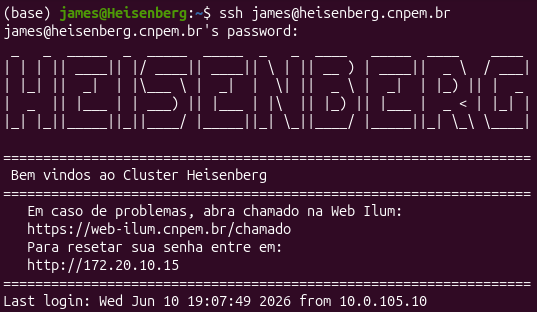
\includegraphics[width=0.85\textwidth]{images/Imagem-Heisenberg-Logada.png}
  \caption{Conexão SSH pelo PowerShell no Windows.}
\end{figure}

\subsection{Reset de Senha}

Caso tenha esquecido sua senha, acesse o portal de reset pelo navegador:
\begin{center}
  \url{http://172.20.10.15}
\end{center}

\begin{atencao}
  O portal de reset de senha só é acessível dentro da rede da Ilum ou via VPN.
\end{atencao}

\subsection{Abertura de Chamados}

Para reportar problemas técnicos, solicitar novos softwares ou tirar dúvidas
com a equipe de TI, utilize o sistema de chamados:
\begin{center}
  \url{https://web-ilum.cnpem.br/chamado}
\end{center}

% =====================================================================
\section{Tutorial de Linux para Iniciantes}
% =====================================================================

\begin{info}
  Esta seção é voltada para quem nunca usou um terminal antes. Se você já tem
  experiência com Linux, pode pular para a Seção~\ref{sec:modulos}.
\end{info}

\subsection{O que é o Terminal?}

O terminal (também chamado de \textit{shell} ou \textit{linha de comando}) é uma
interface de texto onde você digita comandos para o computador executar. No
cluster, \textbf{toda interação é feita pelo terminal} --- não há área de
trabalho gráfica.

Após o login, você verá algo como:

\begin{lstlisting}[style=terminal]
usuario@heisenberg:~$
\end{lstlisting}

Isso significa: \texttt{usuario} = seu nome de usuário;
\texttt{heisenberg} = nome da máquina; \texttt{\textasciitilde} = você está
na sua pasta pessoal (\textit{home}); \texttt{\$} = pronto para receber comandos.

\subsection{Navegando pelo Sistema de Arquivos}

O Linux organiza arquivos em uma árvore de diretórios. A raiz é \texttt{/}.
Sua pasta pessoal fica em \texttt{/home/seu\_usuario} e pode ser referenciada
pelo atalho \texttt{\textasciitilde}.

\subsubsection{Saber onde você está}

\begin{lstlisting}[style=terminal]
$ pwd
/home/joao
\end{lstlisting}

\cmd{pwd} (\textit{print working directory}) mostra o diretório atual.

\subsubsection{Listar arquivos}

\begin{lstlisting}[style=terminal]
$ ls
dados/  scripts/  simulacao.sh

$ ls -lh
total 12K
drwxr-xr-x 2 joao joao 4096 jun  1 10:00 dados
drwxr-xr-x 2 joao joao 4096 jun  1 10:01 scripts
-rw-r--r-- 1 joao joao  512 jun  3 14:22 simulacao.sh
\end{lstlisting}

\texttt{-l} exibe detalhes (permissões, tamanho, data); \texttt{-h} exibe
tamanhos legíveis (KB, MB).

\subsubsection{Entrar em um diretório}

\begin{lstlisting}[style=terminal]
$ cd dados
$ pwd
/home/joao/dados

$ cd ..          # volta um nivel acima
$ cd ~           # volta para a home
$ cd -           # volta para o diretorio anterior
\end{lstlisting}

\subsubsection{Criar diretórios}

\begin{lstlisting}[style=terminal]
$ mkdir meu_projeto
$ mkdir -p meu_projeto/resultados/graficos   # cria toda a arvore
\end{lstlisting}

\subsection{Manipulação de Arquivos}

\subsubsection{Criar um arquivo de texto}

\begin{lstlisting}[style=terminal]
$ nano meu_arquivo.txt
\end{lstlisting}

O \cmd{nano} é um editor de texto simples que funciona direto no terminal.

\begin{figure}[H]
  \centering
  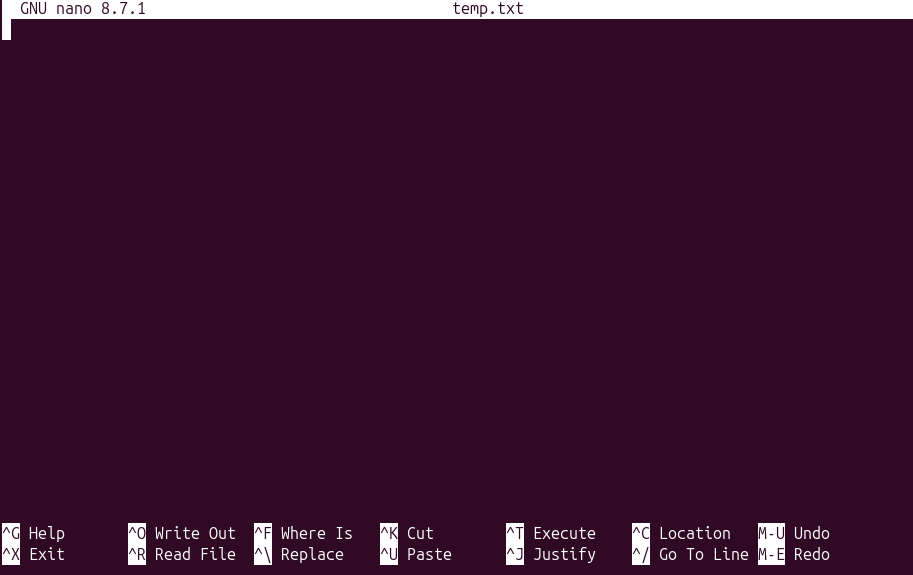
\includegraphics[width=0.85\textwidth]{images/nano.png}
  \caption{Editor de texto \texttt{nano} no terminal.}
\end{figure}

Atalhos do \cmd{nano}:
\begin{itemize}
  \item \texttt{Ctrl+O} $\rightarrow$ salvar (\textit{O de Output})
  \item \texttt{Ctrl+X} $\rightarrow$ sair
  \item \texttt{Ctrl+W} $\rightarrow$ buscar texto
\end{itemize}

\subsubsection{Visualizar conteúdo de arquivos}

\begin{lstlisting}[style=terminal]
$ cat arquivo.txt          # exibe o arquivo inteiro
$ less arquivo.txt         # paginado (q para sair, /termo para buscar)
$ head -20 arquivo.txt     # primeiras 20 linhas
$ tail -20 arquivo.txt     # ultimas 20 linhas
$ tail -f log.out          # acompanha o arquivo em tempo real
\end{lstlisting}

\subsubsection{Copiar, mover e remover}

\begin{lstlisting}[style=terminal]
$ cp arquivo.txt copia.txt          # copiar arquivo
$ cp -r pasta/ pasta_backup/        # copiar pasta inteira
$ mv arquivo.txt novo_nome.txt      # renomear ou mover
$ mv arquivo.txt /home/joao/dados/  # mover para outra pasta

$ rm arquivo.txt                    # remover arquivo
$ rm -r pasta/                      # remover pasta e tudo dentro
\end{lstlisting}

\begin{perigo}
  O comando \cmd{rm} apaga arquivos \textbf{permanentemente} no Linux --- não
  existe lixeira no terminal. Use com muito cuidado, especialmente com
  \texttt{-r} (recursivo). Nunca execute \texttt{rm -rf /} ou
  \texttt{rm -rf *} sem ter certeza absoluta do que está fazendo.
\end{perigo}

\subsection{Transferência de Arquivos}

Os comandos abaixo são digitados no \textbf{terminal do seu próprio computador}
(PowerShell no Windows ou terminal no Linux/macOS), \textbf{não} no cluster.

\subsubsection{Enviar arquivos para o cluster}

\begin{lstlisting}[style=terminal]
# Enviar um arquivo para a home do cluster
$ scp foo.bar seu_usuario@heisenberg.cnpem.br:~/

# Enviar um arquivo para uma subpasta especifica
$ scp foo.bar seu_usuario@heisenberg.cnpem.br:~/dados/

# Enviar uma pasta inteira (-r de recursivo)
$ scp -r minha_pasta/ seu_usuario@heisenberg.cnpem.br:~/
\end{lstlisting}

\subsubsection{Baixar arquivos do cluster}

\begin{lstlisting}[style=terminal]
# Baixar um arquivo para o diretorio atual
$ scp james@heisenberg.cnpem.br:~/foo.bar ./

# Baixar um arquivo de uma subpasta
$ scp james@heisenberg.cnpem.br:~/resultados/output.dat ./

# Baixar uma pasta inteira
$ scp -r james@heisenberg.cnpem.br:~/resultados/ ./
\end{lstlisting}

\begin{dica}
  No Windows, esses comandos funcionam exatamente da mesma forma dentro do
  PowerShell. Não é necessário nenhum programa adicional.
\end{dica}

\subsubsection{Transferência com Interface Gráfica: WinSCP (Windows)}

Para quem prefere uma interface gráfica de arrastar e soltar, o
\textbf{WinSCP} é uma alternativa prática no Windows. Ele permite navegar
pelas pastas do cluster e transferir arquivos sem usar o terminal.

\begin{figure}[H]
  \centering
  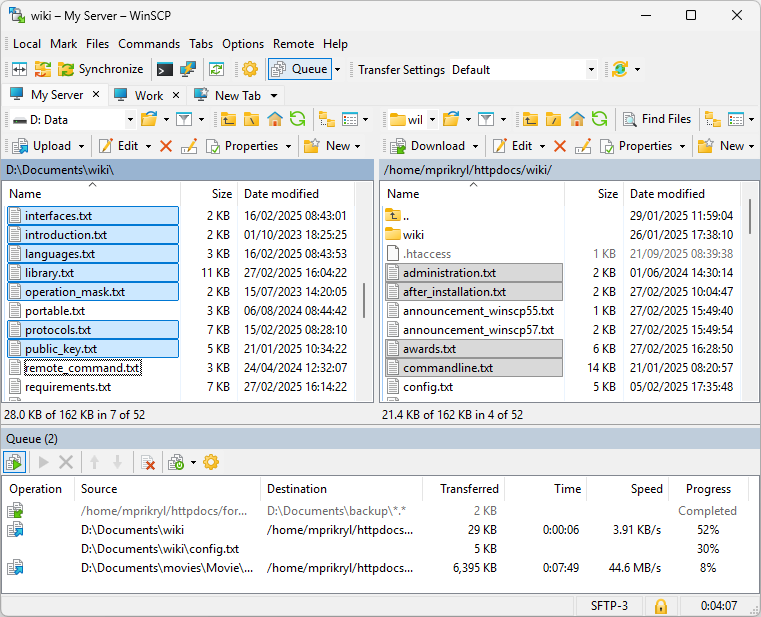
\includegraphics[width=0.85\textwidth]{images/WinSCP.png}
  \caption{WinSCP: transferência de arquivos com interface gráfica.}
\end{figure}

Para um tutorial completo de instalação e uso do WinSCP com o Heisenberg,
assista ao vídeo:

\begin{center}
  \url{https://www.youtube.com/watch?v=2_rJNksIYjk}
\end{center}

\subsection{Processos e Monitoramento}

\begin{lstlisting}[style=terminal]
$ top               # monitor de processos em tempo real (q para sair)
$ htop              # versao melhorada do top (se disponivel)
$ ps aux | grep meu_usuario   # listar seus processos
$ kill 12345        # encerrar processo com PID 12345
\end{lstlisting}

\subsection{Busca e Filtros}

\begin{lstlisting}[style=terminal]
$ grep "erro" log.out          # busca a palavra "erro" no arquivo
$ grep -r "funcao" scripts/    # busca recursiva em uma pasta
$ find . -name "*.py"          # encontra arquivos .py a partir do diretorio atual
$ wc -l arquivo.txt            # conta linhas de um arquivo
\end{lstlisting}

\subsection{Redirecionamento e Pipes}

\begin{lstlisting}[style=terminal]
$ ls -lh > lista.txt         # redireciona saida para arquivo (sobrescreve)
$ ls -lh >> lista.txt        # redireciona e acrescenta ao arquivo
$ cat log.out | grep "ERRO"  # filtra linhas com "ERRO" do log
$ sort numeros.txt | uniq    # ordena e remove duplicatas
\end{lstlisting}

\subsection{Dicas de Produtividade no Terminal}

\begin{dica}
\begin{itemize}[noitemsep]
  \item \textbf{Tab} --- completa automaticamente nomes de arquivos e comandos.
  \item \textbf{Seta $\uparrow$/$\downarrow$} --- navega pelo histórico de comandos.
  \item \textbf{PageUp / PageDown} --- busca no histórico pelo que já foi digitado.
        Por exemplo, se você digitar \texttt{srun} e pressionar \textbf{PageUp},
        o terminal mostrará o último comando que começava com \texttt{srun}.
  \item \textbf{Ctrl+C} --- cancela o comando em execução.
  \item \textbf{Ctrl+L} --- limpa a tela.
  \item \textbf{Ctrl+A} / \textbf{Ctrl+E} --- vai para o início/fim da linha.
  \item \cmd{history} --- exibe os últimos comandos digitados.
  \item \cmd{man ls} --- exibe o manual de qualquer comando (\texttt{q} para sair).
\end{itemize}
\end{dica}

% =====================================================================
\section{Environment Modules}
\label{sec:modulos}
% =====================================================================

O sistema de \textbf{Environment Modules} permite carregar e descarregar
softwares científicos de forma isolada, sem conflitos entre versões.
Quando você carrega um módulo, o sistema ajusta automaticamente variáveis
como \texttt{PATH}, \texttt{LD\_LIBRARY\_PATH} e outras necessárias para
o software funcionar.

\subsection{Comandos Básicos de Módulos}

\begin{lstlisting}[style=terminal]
$ module avail              # lista todos os modulos disponiveis
$ module avail gromacs      # filtra por nome
$ module load gromacs/2026.0  # carrega o modulo
$ module list               # mostra modulos carregados
$ module unload gromacs/2026.0  # descarrega o modulo
$ module purge              # descarrega todos os modulos
$ module show gromacs/2026.0   # exibe o que o modulo configura
$ module help               # ajuda
\end{lstlisting}

\subsection{Módulos Disponíveis no Heisenberg}

\subsubsection{Aplicações Científicas (\texttt{apps})}

\begin{longtable}{lll}
  \toprule
  \textbf{Módulo} & \textbf{Versão} & \textbf{Descrição} \\
  \midrule
  \endhead
  \texttt{amber} & 2024 & Simulação de dinâmica molecular (biomoléculas) \\
  \texttt{gromacs} & 2026.0 & Dinâmica molecular de alta performance \\
  \texttt{ORCA} & 6.1.1 & Química quântica ab initio / DFT \\
  \texttt{quantum-espresso} & 7.5 & DFT para sólidos e superfícies \\
  \texttt{quantum-espresso} & 7.5-aocl & Idem, otimizado com AOCL \\
  \texttt{vasp} & 6.2.0 & Simulação ab initio de materiais \\
  \texttt{vasp} & 6.2.0-aocl & Idem, otimizado com AOCL \\
  \bottomrule
  \caption{Aplicações científicas disponíveis.}
\end{longtable}

\subsubsection{Bibliotecas e Compiladores (\texttt{libraries})}

\begin{longtable}{lll}
  \toprule
  \textbf{Módulo} & \textbf{Versão} & \textbf{Descrição} \\
  \midrule
  \endhead
  \texttt{cuda} & 12.4, 13.1 & NVIDIA CUDA Toolkit (programação GPU) \\
  \texttt{aocl} & 5.3.0 / 5.3.0-mt / 5.3.0-st & AMD Optimizing CPU Libraries \\
  \texttt{elpa} & 2024.05.001 & Eigenvalue SoLvers para HPC \\
  \texttt{hwloc} & 2.12.2 & Topologia de hardware \\
  \texttt{intel/compiler} & 2025.3.0 & Intel oneAPI C/C++/Fortran \\
  \texttt{intel/compiler-intel-llvm} & 2025.3.0 & Intel LLVM compiler \\
  \texttt{intel/mkl} & 2025.3 & Intel Math Kernel Library \\
  \texttt{intel/mpi} & 2021.17 & Intel MPI \\
  \texttt{intel/tbb} & 2022.3 & Intel Threading Building Blocks \\
  \texttt{intel/dnnl} & 3.9.1 & Deep Neural Network Library \\
  \texttt{intel/debugger} & 2025.3.0 & Intel Debugger \\
  \texttt{openmpi} & 4.1.8, 5.0.9 & Open MPI (comunicação entre processos) \\
  \texttt{pmix} & 5.0.9 & Process Management Interface \\
  \texttt{scalapack} & 2.2.0-ompi509 & ScaLAPACK (álgebra linear paralela) \\
  \bottomrule
  \caption{Bibliotecas e compiladores disponíveis.}
\end{longtable}

\subsection{Exemplo: Carregando o GROMACS}

\begin{lstlisting}[style=terminal]
$ module load gromacs/2026.0
$ gmx --version
\end{lstlisting}

\begin{dica}
  Para garantir que o ambiente correto seja carregado toda vez que você fizer
  login, adicione o comando \cmd{module load} ao arquivo \texttt{\textasciitilde/.bashrc}:
  \begin{lstlisting}[style=terminal]
$ nano ~/.bashrc
# Adicione ao final:
module load gromacs/2026.0
  \end{lstlisting}
\end{dica}

% =====================================================================
\section{Python com Miniconda}
\label{sec:python}
% =====================================================================

\textbf{Miniconda} é um instalador minimalista do gerenciador de pacotes
\textbf{conda}. Ele permite criar \textbf{ambientes virtuais} isolados, onde
cada projeto pode ter sua própria versão do Python e suas próprias bibliotecas,
sem interferir no sistema ou em outros projetos.

\begin{info}
  O Miniconda é instalado \textbf{na sua área pessoal} (\texttt{\textasciitilde/}),
  sem necessidade de permissão de administrador. Cada usuário instala e gerencia
  seu próprio ambiente.
\end{info}

\subsection{Instalando o Miniconda}

\textbf{Passo 1 — Baixar o instalador:}

\begin{lstlisting}[style=terminal]
$ wget https://repo.anaconda.com/miniconda/Miniconda3-latest-Linux-x86_64.sh
\end{lstlisting}

\textbf{Passo 2 — Executar o instalador:}

\begin{lstlisting}[style=terminal]
$ bash Miniconda3-latest-Linux-x86_64.sh
\end{lstlisting}

O instalador fará algumas perguntas:
\begin{itemize}
  \item \textbf{Do you accept the license terms?} $\rightarrow$ Digite \texttt{yes} e pressione
        \texttt{Enter}.
  \item \textbf{Confirm install location} $\rightarrow$ Pressione \texttt{Enter} para aceitar
        o padrão (\texttt{\textasciitilde/miniconda3}).
  \item \textbf{Do you wish the installer to initialize Miniconda3?} $\rightarrow$ Digite
        \texttt{yes} e pressione \texttt{Enter}. Isso configura o conda
        automaticamente no seu shell.
\end{itemize}

\textbf{Passo 3 — Recarregar o shell:}

\begin{lstlisting}[style=terminal]
$ source ~/.bashrc
\end{lstlisting}

Após isso, o prompt mostrará \texttt{(base)} antes do seu nome de usuário,
indicando que o conda está ativo.

\textbf{Passo 4 — Verificar a instalação:}

\begin{lstlisting}[style=terminal]
$ conda --version
conda 24.x.x
\end{lstlisting}

\subsection{Criando o Ambiente \texttt{ilumpy}}

Com o conda instalado, crie um ambiente dedicado com Python 3.11:

\begin{lstlisting}[style=terminal]
$ conda create -n ilumpy python=3.11
\end{lstlisting}

O conda listará os pacotes que serão instalados e pedirá confirmação.
Digite \texttt{y} e pressione \texttt{Enter}.

\textbf{Ative o ambiente:}

\begin{lstlisting}[style=terminal]
$ conda activate ilumpy
\end{lstlisting}

O prompt mudará para \texttt{(ilumpy)}, confirmando que o ambiente está ativo:

\begin{lstlisting}[style=terminal]
(ilumpy) usuario@heisenberg:~$
\end{lstlisting}

\textbf{Verifique a versão do Python:}

\begin{lstlisting}[style=terminal]
$ python --version
Python 3.11.x
\end{lstlisting}

\subsection{Instalando Bibliotecas Científicas via pip}

Com o ambiente \texttt{ilumpy} ativo, instale as bibliotecas mais utilizadas
em Python científico com um único comando:

\begin{lstlisting}[style=terminal]
$ pip install numpy scipy matplotlib pandas seaborn scikit-learn \
              jupyter ipython sympy tqdm h5py pyarrow statsmodels \
              networkx pillow
\end{lstlisting}

A tabela abaixo descreve o propósito de cada biblioteca:

\begin{longtable}{ll}
  \toprule
  \textbf{Biblioteca} & \textbf{Finalidade} \\
  \midrule
  \endhead
  \texttt{numpy} & Arrays numéricos e álgebra linear \\
  \texttt{scipy} & Algoritmos científicos (integração, otimização, estatística) \\
  \texttt{matplotlib} & Geração de gráficos e visualizações \\
  \texttt{pandas} & Manipulação de dados tabulares (DataFrames) \\
  \texttt{seaborn} & Gráficos estatísticos de alta qualidade \\
  \texttt{scikit-learn} & Aprendizado de máquina clássico \\
  \texttt{ipython} & Console Python interativo aprimorado \\
  \texttt{sympy} & Matemática simbólica \\
  \texttt{tqdm} & Barras de progresso em loops \\
  \texttt{h5py} & Leitura/escrita de arquivos HDF5 \\
  \texttt{pyarrow} & Leitura/escrita de arquivos Parquet e Arrow \\
  \texttt{statsmodels} & Modelos estatísticos e econométricos \\
  \texttt{networkx} & Análise de grafos e redes \\
  \texttt{pillow} & Processamento de imagens \\
  \bottomrule
  \caption{Bibliotecas Python instaladas no ambiente \texttt{ilumpy}.}
\end{longtable}

\subsection{Ativando o Ambiente Automaticamente}

Para não precisar digitar \cmd{conda activate ilumpy} a cada login, adicione
a ativação ao arquivo \texttt{\textasciitilde/.bashrc}:

\begin{lstlisting}[style=terminal]
$ nano ~/.bashrc
\end{lstlisting}

Adicione a linha abaixo ao final do arquivo:

\begin{lstlisting}[style=terminal]
conda activate ilumpy
\end{lstlisting}

Salve com \texttt{Ctrl+O} e saia com \texttt{Ctrl+X}. Na próxima vez que fizer
login, o ambiente \texttt{ilumpy} já estará ativo.

\subsection{Comandos Úteis do Conda}

\begin{lstlisting}[style=terminal]
$ conda activate ilumpy      # ativa o ambiente
$ conda deactivate           # desativa (volta para base)
$ conda env list             # lista todos os ambientes
$ conda list                 # lista pacotes do ambiente ativo
$ pip list                   # idem, para pacotes instalados via pip
$ pip install nome_pacote    # instala novo pacote
$ pip show numpy             # informacoes sobre um pacote
\end{lstlisting}

\begin{dica}
  Sempre ative o ambiente correto \textbf{antes} de submeter um job que
  rode Python. No script \texttt{.sh}, inclua \cmd{conda activate ilumpy}
  logo após carregar os módulos necessários. Veja os exemplos na
  Seção~\ref{sec:jobs_python}.
\end{dica}

% =====================================================================
\section{Gerenciador de Filas Slurm}
\label{sec:slurm}
% =====================================================================

O \textbf{Slurm} é o software que gerencia e distribui os recursos do cluster
entre os usuários. Você não executa seus programas diretamente; em vez disso,
escreve um \textbf{script de job} que descreve os recursos necessários
(CPUs, memória, tempo, GPUs) e o submete à fila. O Slurm decide quando e
em qual nó o job irá rodar.

\subsection{Filas (Partitions) Disponíveis}

\begin{longtable}{lllrl}
  \toprule
  \textbf{Fila} & \textbf{Default} & \textbf{Nós} & \textbf{CPUs Totais} & \textbf{Obs.} \\
  \midrule
  \endhead
  \texttt{cpu} & Sim & work0--3, work7 & 416 & Apenas CPU \\
  \texttt{gpu} & Não & work1, work4--6, work8 & 224 & CPU + GPU \\
  \bottomrule
  \caption{Partições (filas) do Cluster Heisenberg.}
\end{longtable}

\begin{atencao}
  A fila \texttt{cpu} é a padrão. Se seu job precisar de GPU, especifique
  explicitamente \texttt{--partition=gpu} e \texttt{--gres=gpu:1} no script.
\end{atencao}

\subsection{Comandos Essenciais do Slurm}

\begin{longtable}{ll}
  \toprule
  \textbf{Comando} & \textbf{Função} \\
  \midrule
  \endhead
  \cmd{sinfo} & Ver estado das filas e nós \\
  \cmd{squeue} & Ver jobs na fila \\
  \cmd{sbatch script.sh} & Submeter um job (modo batch) \\
  \cmd{srun} & Executar interativamente \\
  \cmd{scancel JOBID} & Cancelar um job \\
  \cmd{sacct} & Ver histórico de jobs \\
  \cmd{scontrol show job JOBID} & Detalhes de um job específico \\
  \bottomrule
  \caption{Comandos principais do Slurm.}
\end{longtable}

\subsubsection{Verificar estado das filas}

\begin{lstlisting}[style=terminal]
$ sinfo
PARTITION  AVAIL  TIMELIMIT  NODES  STATE   NODELIST
cpu*       up     infinite   2      mix     work[0-1]
cpu*       up     infinite   2      alloc   work[2-3]
gpu        up     infinite   3      mix     work[1,4-5]
gpu        up     infinite   2      idle    work[6,8]
\end{lstlisting}

Os estados dos nós significam:
\begin{itemize}[noitemsep]
  \item \texttt{idle} --- nó livre, pronto para receber jobs;
  \item \texttt{mix} --- parcialmente ocupado (alguns CPUs livres);
  \item \texttt{alloc} --- totalmente ocupado;
  \item \texttt{down} --- nó fora de serviço.
\end{itemize}

\subsubsection{Ver jobs em execução}

\begin{lstlisting}[style=terminal]
$ squeue
JOBID    USER     NAME            PARTITION  STATE   TIME      NODES
9426     joao     simulacao.sh    cpu        RUNNING 40:13     1
9427     maria    analise.sh      gpu        PENDING 0:00      1

$ squeue -u meu_usuario    # apenas seus jobs
\end{lstlisting}

\subsection{Escrevendo um Script de Job}

Um script de job é um arquivo de texto com extensão \texttt{.sh} contendo:
\begin{enumerate}
  \item Diretivas Slurm (iniciadas com \texttt{\#SBATCH});
  \item Comandos para carregar módulos;
  \item O comando do seu programa.
\end{enumerate}

\subsubsection{Parâmetros Principais do \texttt{\#SBATCH}}

\begin{longtable}{ll}
  \toprule
  \textbf{Parâmetro} & \textbf{Descrição} \\
  \midrule
  \endhead
  \texttt{--job-name=nome} & Nome do job (aparece no \cmd{squeue}) \\
  \texttt{--partition=cpu} & Fila a usar (\texttt{cpu} ou \texttt{gpu}) \\
  \texttt{--nodes=1} & Número de nós \\
  \texttt{--ntasks=1} & Número de tarefas MPI \\
  \texttt{--cpus-per-task=8} & CPUs por tarefa (threads OpenMP) \\
  \texttt{--mem=16G} & Memória total por nó \\
  \texttt{--time=12:00:00} & Tempo máximo (HH:MM:SS) \\
  \texttt{--gres=gpu:1} & Solicitar 1 GPU \\
  \texttt{--output=saida.out} & Arquivo de saída padrão \\
  \texttt{--error=erros.err} & Arquivo de erros \\
  \texttt{--mail-type=END,FAIL} & Notificação por e-mail \\
  \texttt{--mail-user=email@ilum.br} & E-mail para notificações \\
  \bottomrule
  \caption{Principais diretivas \texttt{\#SBATCH}.}
\end{longtable}

\subsection{Exemplos de Scripts de Job}

\subsubsection{Job Simples (CPU, serial)}

\begin{lstlisting}[style=script, language=bash]
#!/bin/bash
#SBATCH --job-name=meu_primeiro_job
#SBATCH --partition=cpu
#SBATCH --nodes=1
#SBATCH --ntasks=1
#SBATCH --cpus-per-task=4
#SBATCH --mem=8G
#SBATCH --time=02:00:00
#SBATCH --output=saida_%j.out
#SBATCH --error=erros_%j.err

# Carregar modulos necessarios
module load intel/compiler/2025.3.0

# Executar o programa
echo "Job iniciado: $(date)"
./meu_programa input.dat
echo "Job concluido: $(date)"
\end{lstlisting}

O \texttt{\%j} no nome do arquivo será substituído automaticamente pelo número
do job (JOBID), evitando sobrescrever saídas de execuções anteriores.

\subsubsection{Job com MPI (múltiplos processos)}

\begin{lstlisting}[style=script, language=bash]
#!/bin/bash
#SBATCH --job-name=simulacao_mpi
#SBATCH --partition=cpu
#SBATCH --nodes=2
#SBATCH --ntasks=16
#SBATCH --cpus-per-task=8
#SBATCH --mem=64G
#SBATCH --time=24:00:00
#SBATCH --output=mpi_%j.out
#SBATCH --error=mpi_%j.err

module load openmpi/5.0.9
module load intel/mkl/2025.3

srun ./programa_mpi input.dat
\end{lstlisting}

\subsubsection{Job com GPU}

\begin{lstlisting}[style=script, language=bash]
#!/bin/bash
#SBATCH --job-name=treinamento_gpu
#SBATCH --partition=gpu
#SBATCH --nodes=1
#SBATCH --ntasks=1
#SBATCH --cpus-per-task=8
#SBATCH --gres=gpu:1
#SBATCH --mem=32G
#SBATCH --time=08:00:00
#SBATCH --output=gpu_%j.out
#SBATCH --error=gpu_%j.err

module load cuda/12.4

echo "GPU disponivel:"
nvidia-smi

python treinar_modelo.py --epochs 100
\end{lstlisting}

\subsubsection{Job GROMACS (exemplo completo)}

\begin{lstlisting}[style=script, language=bash]
#!/bin/bash
#SBATCH --job-name=gromacs_md
#SBATCH --partition=cpu
#SBATCH --nodes=1
#SBATCH --ntasks=1
#SBATCH --cpus-per-task=32
#SBATCH --mem=64G
#SBATCH --time=48:00:00
#SBATCH --output=gromacs_%j.out
#SBATCH --error=gromacs_%j.err
#SBATCH --mail-type=END,FAIL
#SBATCH --mail-user=meu@email.com.br

module load gromacs/2026.0

export OMP_NUM_THREADS=$SLURM_CPUS_PER_TASK

# Etapa de equilibracao
gmx mdrun -v -deffnm equilibracao -ntmpi 1 \
          -ntomp $OMP_NUM_THREADS

# Producao
gmx mdrun -v -deffnm producao -ntmpi 1 \
          -ntomp $OMP_NUM_THREADS
\end{lstlisting}

\subsubsection{Job VASP}

\begin{lstlisting}[style=script, language=bash]
#!/bin/bash
#SBATCH --job-name=vasp_dft
#SBATCH --partition=cpu
#SBATCH --nodes=1
#SBATCH --ntasks=32
#SBATCH --mem=128G
#SBATCH --time=72:00:00
#SBATCH --output=vasp_%j.out
#SBATCH --error=vasp_%j.err

module load vasp/6.2.0

mpirun -np $SLURM_NTASKS vasp_std
\end{lstlisting}

% ------------------------------------------------------------------
\subsection{Jobs Python}
\label{sec:jobs_python}
% ------------------------------------------------------------------

\begin{info}
  \textbf{Python é serial por padrão.} O interpretador CPython possui uma
  trava interna chamada \textbf{GIL} (\textit{Global Interpreter Lock}) que
  impede a execução simultânea de múltiplos \textit{threads} Python no mesmo
  processo. Isso significa que, na maior parte dos casos, um script Python
  utiliza \textbf{apenas 1 CPU} por vez, independentemente de quantas CPUs
  você reserve no Slurm.

  O comportamento muda quando o script usa bibliotecas que realizam
  processamento paralelo internamente, como:
  \begin{itemize}[noitemsep]
    \item \textbf{NumPy / SciPy / scikit-learn} --- operações vetorizadas
          podem usar múltiplos núcleos via BLAS/OpenBLAS em background;
    \item \textbf{multiprocessing} / \textbf{joblib} / \textbf{concurrent.futures}
          --- paralelismo explícito usando múltiplos processos;
    \item \textbf{PyTorch} / \textbf{TensorFlow} (com GPU) --- treinamento
          em GPU requer a fila \texttt{gpu} e \texttt{--gres=gpu:1}.
  \end{itemize}
  Se o seu script não usa nenhuma dessas estratégias, solicite
  \textbf{apenas 1 CPU} e não desperdice recursos do cluster.
\end{info}

\subsubsection{Job Python Serial}

Use este modelo para scripts que \textbf{não} utilizam paralelismo explícito.
A flag \texttt{-u} no comando Python desativa o buffer de saída, garantindo
que as mensagens apareçam no arquivo de saída em tempo real (sem atraso).

\begin{lstlisting}[style=script, language=bash]
#!/bin/bash
#SBATCH --job-name=python_serial
#SBATCH --partition=cpu
#SBATCH --nodes=1
#SBATCH --ntasks=1
#SBATCH --cpus-per-task=1
#SBATCH --mem=1G
#SBATCH --time=04:00:00
#SBATCH --output=python_%j.out
#SBATCH --error=python_%j.err

# Ativa o ambiente Python com as bibliotecas instaladas
source ~/.bashrc
conda activate ilumpy

echo "Inicio: $(date)"
echo "No: $(hostname)"

# -u: saida sem buffer (aparece em tempo real no arquivo .out)
python -u script.py > script.out

echo "Fim: $(date)"
\end{lstlisting}

\begin{dica}
  O redirecionamento \texttt{> script.out} grava a saída do \emph{print}
  do Python em \texttt{script.out}, enquanto erros e exceções vão para o
  arquivo \texttt{.err} definido no \texttt{\#SBATCH}. Assim você tem os
  resultados e os erros separados, facilitando a depuração.
\end{dica}

\subsubsection{Job Python Paralelo}

Use este modelo quando o script utiliza múltiplos processos ou threads
para aproveitar mais de um núcleo --- por exemplo com \texttt{multiprocessing},
\texttt{joblib} ou operações pesadas de NumPy/SciPy que usam BLAS em paralelo.

\begin{lstlisting}[style=script, language=bash]
#!/bin/bash
#SBATCH --job-name=python_paralelo
#SBATCH --partition=cpu
#SBATCH --nodes=1
#SBATCH --ntasks=1
#SBATCH --cpus-per-task=16
#SBATCH --mem=32G
#SBATCH --time=08:00:00
#SBATCH --output=python_%j.out
#SBATCH --error=python_%j.err

conda activate ilumpy

# Informa ao script quantas CPUs foram alocadas pelo Slurm
export N_CPUS=$SLURM_CPUS_PER_TASK

echo "Inicio: $(date)"
echo "No: $(hostname)"
echo "CPUs disponiveis: $N_CPUS"

python -u script.py > script.out

echo "Fim: $(date)"
\end{lstlisting}

No script Python, leia a variável de ambiente para saber quantos núcleos
usar:

\begin{lstlisting}[style=script, language=Python]
import os
from joblib import Parallel, delayed

n_cpus = int(os.environ.get("N_CPUS", 1))
print(f"Usando {n_cpus} CPUs")

# Exemplo com joblib: executa 'minha_funcao' em paralelo
resultados = Parallel(n_jobs=n_cpus)(
    delayed(minha_funcao)(i) for i in range(100)
)
\end{lstlisting}

\begin{atencao}
  Solicite apenas o número de CPUs que seu código \textbf{realmente} vai
  usar. Alocar 16 CPUs para um script serial desperdiça recursos e atrasa
  outros usuários na fila. Em caso de dúvida, comece com 1 CPU e aumente
  conforme necessário após verificar com \cmd{sacct}.
\end{atencao}

\subsection{Submetendo e Acompanhando o Job}

\begin{lstlisting}[style=terminal]
# Submeter o job
$ sbatch meu_script.sh
Submitted batch job 9430

# Verificar se esta na fila
$ squeue -u meu_usuario
JOBID  USER  NAME              STATE    TIME
9430   joao  meu_primeiro_job  PENDING  0:00

# Acompanhar a saida em tempo real
$ tail -f saida_9430.out

# Cancelar o job
$ scancel 9430
\end{lstlisting}

\subsection{Sessão Interativa}

Para testar comandos, depurar scripts ou usar programas interativos,
solicite uma sessão interativa em vez de submeter um job:

\begin{lstlisting}[style=terminal]
$ srun --partition=cpu --nodes=1 --ntasks=4 --mem=8G \
       --time=01:00:00 --pty bash

# Com GPU:
$ srun --partition=gpu --gres=gpu:1 --ntasks=4 \
       --mem=16G --time=02:00:00 --pty bash
\end{lstlisting}

\begin{atencao}
  Sessões interativas também consomem recursos do cluster. Encerre-as
  com \cmd{exit} assim que terminar o trabalho.
\end{atencao}

\subsection{Variáveis de Ambiente do Slurm}

Dentro do script de job, o Slurm disponibiliza variáveis úteis:

\begin{longtable}{ll}
  \toprule
  \textbf{Variável} & \textbf{Conteúdo} \\
  \midrule
  \endhead
  \texttt{\$SLURM\_JOB\_ID} & ID do job \\
  \texttt{\$SLURM\_JOB\_NAME} & Nome do job \\
  \texttt{\$SLURM\_NTASKS} & Número total de tarefas \\
  \texttt{\$SLURM\_CPUS\_PER\_TASK} & CPUs por tarefa \\
  \texttt{\$SLURM\_MEM\_PER\_NODE} & Memória por nó (MB) \\
  \texttt{\$SLURM\_NODELIST} & Lista de nós alocados \\
  \texttt{\$SLURM\_SUBMIT\_DIR} & Diretório de onde sbatch foi chamado \\
  \bottomrule
  \caption{Variáveis de ambiente do Slurm.}
\end{longtable}

% =====================================================================
\section{Boas Práticas}
% =====================================================================

\subsection{Organização de Arquivos}

Mantenha sua área de trabalho organizada. Uma estrutura sugerida:

\begin{lstlisting}[style=terminal]
~/
|-- projetos/
|   |-- simulacao_proteina/
|   |   |-- input/
|   |   |-- output/
|   |   |-- scripts/
|   |   `-- logs/
|   `-- calculo_dft/
|       |-- ...
`-- scripts_uteis/
\end{lstlisting}

\subsection{Estimativa de Recursos}

\begin{itemize}
  \item Comece com jobs pequenos para calibrar o tempo de execução.
  \item Não solicite mais memória ou CPUs do que seu programa realmente usa.
  \item Monitore o uso real com \cmd{sstat} ou \cmd{sacct} após o job terminar.
\end{itemize}

\begin{lstlisting}[style=terminal]
$ sacct -j 9430 --format=JobID,Elapsed,CPUTime,MaxRSS,State
\end{lstlisting}

\subsection{Cotas e Limites}

Cada estudante pode utilizar até \textbf{16 CPUs simultâneas} no cluster.
Casos excepcionais que demandem mais recursos podem ser avaliados pela equipe
de TI mediante abertura de chamado em
\url{https://web-ilum.cnpem.br/chamado}.

\subsection{Etiqueta no Uso do Cluster}

\begin{enumerate}
  \item \textbf{Nunca} execute jobs pesados no nó de login.
  \item Estime o tempo necessário e coloque \texttt{--time} realista (nem muito
        apertado, nem exagerado).
  \item Cancele jobs com \cmd{scancel} se perceber que não precisará mais deles.
  \item Remova arquivos temporários e de saída desnecessários regularmente.
  \item Em caso de dúvidas técnicas ou problemas, abra um chamado em
        \url{https://web-ilum.cnpem.br/chamado}.
\end{enumerate}

% =====================================================================
\section{Guia Rápido de Referência}
% =====================================================================

\subsection{Cheatsheet de Linux}

\begin{longtable}{ll}
  \toprule
  \textbf{Comando} & \textbf{O que faz} \\
  \midrule
  \endhead
  \cmd{pwd} & Mostra o diretório atual \\
  \cmd{ls -lh} & Lista arquivos com detalhes \\
  \cmd{cd pasta/} & Entra na pasta \\
  \cmd{cd ..} & Volta um nível \\
  \cmd{mkdir nome} & Cria diretório \\
  \cmd{cp a b} & Copia arquivo a para b \\
  \cmd{mv a b} & Move/renomeia a para b \\
  \cmd{rm arquivo} & Remove arquivo \\
  \cmd{nano arquivo} & Edita arquivo \\
  \cmd{cat arquivo} & Exibe arquivo \\
  \cmd{less arquivo} & Exibe com paginação \\
  \cmd{grep "texto" arq} & Busca texto no arquivo \\
  \cmd{scp arq user@host:dir/} & Envia arquivo via SSH \\
  \cmd{Ctrl+C} & Cancela comando atual \\
  \cmd{Tab} & Autocompleta \\
  \cmd{man comando} & Manual do comando \\
  \bottomrule
  \caption{Referência rápida de comandos Linux.}
\end{longtable}

\subsection{Cheatsheet do Slurm}

\begin{longtable}{ll}
  \toprule
  \textbf{Comando} & \textbf{O que faz} \\
  \midrule
  \endhead
  \cmd{sinfo} & Estado das filas e nós \\
  \cmd{squeue} & Jobs na fila \\
  \cmd{squeue -u usuario} & Seus jobs \\
  \cmd{sbatch script.sh} & Submeter job \\
  \cmd{scancel JOBID} & Cancelar job \\
  \cmd{scontrol show job JOBID} & Detalhes do job \\
  \cmd{sacct -j JOBID} & Histórico e uso de recursos \\
  \cmd{srun --pty bash} & Sessão interativa \\
  \bottomrule
  \caption{Referência rápida de comandos Slurm.}
\end{longtable}

\subsection{Cheatsheet de Módulos}

\begin{longtable}{ll}
  \toprule
  \textbf{Comando} & \textbf{O que faz} \\
  \midrule
  \endhead
  \cmd{module avail} & Lista módulos disponíveis \\
  \cmd{module load nome/versao} & Carrega módulo \\
  \cmd{module list} & Módulos carregados \\
  \cmd{module unload nome} & Descarrega módulo \\
  \cmd{module purge} & Descarrega todos \\
  \cmd{module show nome} & Mostra o que o módulo altera \\
  \bottomrule
  \caption{Referência rápida de Environment Modules.}
\end{longtable}

\subsection{Cheatsheet do Conda / Python}

\begin{longtable}{ll}
  \toprule
  \textbf{Comando} & \textbf{O que faz} \\
  \midrule
  \endhead
  \cmd{conda activate ilumpy} & Ativa o ambiente \texttt{ilumpy} \\
  \cmd{conda deactivate} & Desativa o ambiente atual \\
  \cmd{conda env list} & Lista todos os ambientes \\
  \cmd{conda list} & Lista pacotes do ambiente ativo \\
  \cmd{pip install pacote} & Instala pacote no ambiente ativo \\
  \cmd{pip list} & Lista pacotes instalados via pip \\
  \cmd{pip show pacote} & Informações sobre um pacote \\
  \cmd{python -u script.py} & Executa Python sem buffer de saída \\
  \cmd{python -u script.py > out} & Redireciona saída para arquivo \\
  \bottomrule
  \caption{Referência rápida de Conda e Python.}
\end{longtable}

% =====================================================================
\section{Suporte e Contato}
% =====================================================================

\begin{tcolorbox}[colback=infoblue, colframe=infoborder,
                  title={Onde buscar ajuda}, fonttitle=\bfseries]
\begin{description}
  \item[Sistema de chamados:] \url{https://web-ilum.cnpem.br/chamado}\\
    Use para relatar problemas técnicos, solicitar instalação de software,
    pedir aumento de cota ou qualquer dificuldade com o cluster.
  \item[Reset de senha:] \url{http://172.20.10.15}\\
    Acesse dentro da rede Ilum ou via VPN para redefinir sua senha.
  \item[Endereço do cluster:] \texttt{heisenberg.cnpem.br}
\end{description}
\end{tcolorbox}

\vspace{1em}

Ao abrir um chamado, inclua sempre:
\begin{itemize}
  \item Seu nome de usuário;
  \item O JOBID do job com problema (se aplicável);
  \item A mensagem de erro completa;
  \item O conteúdo do arquivo \texttt{.err} gerado pelo job.
\end{itemize}

% =====================================================================
% Apêndice
% =====================================================================
\appendix

\section{Glossário}

\begin{description}[style=nextline]
  \item[Cluster] Conjunto de computadores interconectados que trabalham como
    uma única máquina.
  \item[CPU (\textit{Central Processing Unit})] Processador central; realiza
    cálculos de propósito geral.
  \item[Ambiente Virtual (conda/venv)] Espaço isolado com versão própria
    do Python e bibliotecas, sem interferir no sistema ou em outros projetos.
  \item[conda] Gerenciador de pacotes e ambientes virtuais; base do Miniconda
    e Anaconda.
  \item[GIL (\textit{Global Interpreter Lock})] Trava do CPython que impede
    execução simultânea de múltiplos \textit{threads} Python; torna scripts
    comuns essencialmente seriais.
  \item[GPU (\textit{Graphics Processing Unit})] Processador gráfico; realiza
    cálculos paralelos massivos (ML, simulações GPU).
  \item[HPC (\textit{High-Performance Computing})] Computação de alto
    desempenho.
  \item[Miniconda] Distribuição minimalista do conda; permite instalar o
    gerenciador de pacotes Python sem uma distribuição completa como o Anaconda.
  \item[Job] Tarefa submetida ao Slurm para execução nos nós de trabalho.
  \item[MPI (\textit{Message Passing Interface})] Padrão para comunicação entre
    processos em múltiplos nós.
  \item[Módulo (Environment Module)] Mecanismo para carregar/descarregar
    softwares e suas dependências dinamicamente.
  \item[Nó (\textit{Node})] Cada computador individual dentro do cluster.
  \item[Nó de login (\textit{login node})] Ponto de acesso ao cluster; não deve
    ser usado para cálculos pesados.
  \item[OpenMP] API para paralelismo de memória compartilhada (multithreading).
  \item[Partição (Partition)] Fila de jobs com regras específicas de acesso e
    recursos.
  \item[QOS (\textit{Quality of Service})] Política que limita o uso de recursos
    por usuário ou grupo.
  \item[SSH (\textit{Secure Shell})] Protocolo criptografado para acesso remoto
    a servidores.
  \item[Slurm] Sistema de gerenciamento de recursos e filas de jobs usado no
    Heisenberg.
\end{description}

\section{Checklist do Primeiro Uso}

\begin{enumerate}
  \item[\(\square\)] Obtive minha conta na Ilum/CNPEM.
  \item[\(\square\)] Abri o PowerShell (Windows) ou o terminal (Linux/macOS).
  \item[\(\square\)] Me conectei ao cluster: \texttt{ssh usuario@heisenberg.cnpem.br}.
  \item[\(\square\)] Explorei minha pasta home com \cmd{ls} e \cmd{pwd}.
  \item[\(\square\)] Listei os módulos com \cmd{module avail}.
  \item[\(\square\)] Instalei o Miniconda na minha home.
  \item[\(\square\)] Criei o ambiente \texttt{ilumpy} com Python 3.11.
  \item[\(\square\)] Instalei as bibliotecas científicas com \cmd{pip install}.
  \item[\(\square\)] Verifiquei as filas com \cmd{sinfo}.
  \item[\(\square\)] Escrevi e submeti meu primeiro job com \cmd{sbatch}.
  \item[\(\square\)] Acompanhei o job com \cmd{squeue} e \cmd{tail -f saida.out}.
\end{enumerate}

\end{document}
